\subsection{NIC-Driven Thread Scheduling}
\label{ssec:thread-scheduler}
In some specialized applications, thread scheduling might not be needed: Big HPC applications, for example, might pin a nanoservice to its own core for the duration of a run. But this won't work for a cloud provider who needs more economic sharing of \name{}s by multiple nanoservices.
Nanotask threads will therefore be switched in and out frequently, and context switches must be extremely fast, else we will lose all the low latency benefits of nanoservices.

If \name{} relied on software scheduling it would be too slow. The fastest best-of-breed software schedulers use 5$\mu$s timer interrupts~\cite{shinjuku, shenango} which are much too slow for our $<1\mu$s nanotasks.

And so, instead, \name{} decides which thread to run next in hardware on the NIC, then tells the CPU core. The NIC keeps track of the highest priority nanotask with messages to process and interrupts the CPU to initiate a context switch under two conditions:
\begin{enumerate}
    \item A message arrives for a higher priority context than the one currently running on the core.
    \item The current context tells the NIC it is idle, and the NIC has messages for another context to process. This condition prevents an idle high priority context from starving a low priority context with messages waiting to be processed.
\end{enumerate}

Figure~\ref{fig:nic-scheduler} shows what happens when a message arrives for a higher priority context than the one currently running on the core. In steps 1 and 2, the arriving message is placed in the RX queue for the high priority context. The NIC scheduler tells the CPU that a high priority message is waiting by placing the context ID in the \texttt{ltargetcontext} CSR. In step 3, the NIC scheduler interrupts the CPU, causing a trap into the nanoKernel, which reads the \texttt{ltargetcontext} CSR and performs a switch to the high priority context. At this point, the high priority context is running on the core and is able to process the message in its RX queue.

\nick{I propose we axe this paragraph to save space and update the figure to remove the CDC. it is an implementation detail we don't need here} Note that there may be words in the clock-domain crossing (CDC) FIFO for the low priority context when the NIC initiates a context switch.
Since these words have not yet been read by the low priority context, they must be pushed back into the low priority RX queue.
Fortunately, it is easy to implement a FIFO that is able to ``unread'' the last few words that were read out.

When the high priority context finishes processing the message, it tells the NIC that it is now idle by writing to a dedicated CSR called \texttt{lidle}. The NIC initiates a context switch back to the low priority context because it still has messages to process.

\begin{figure}
  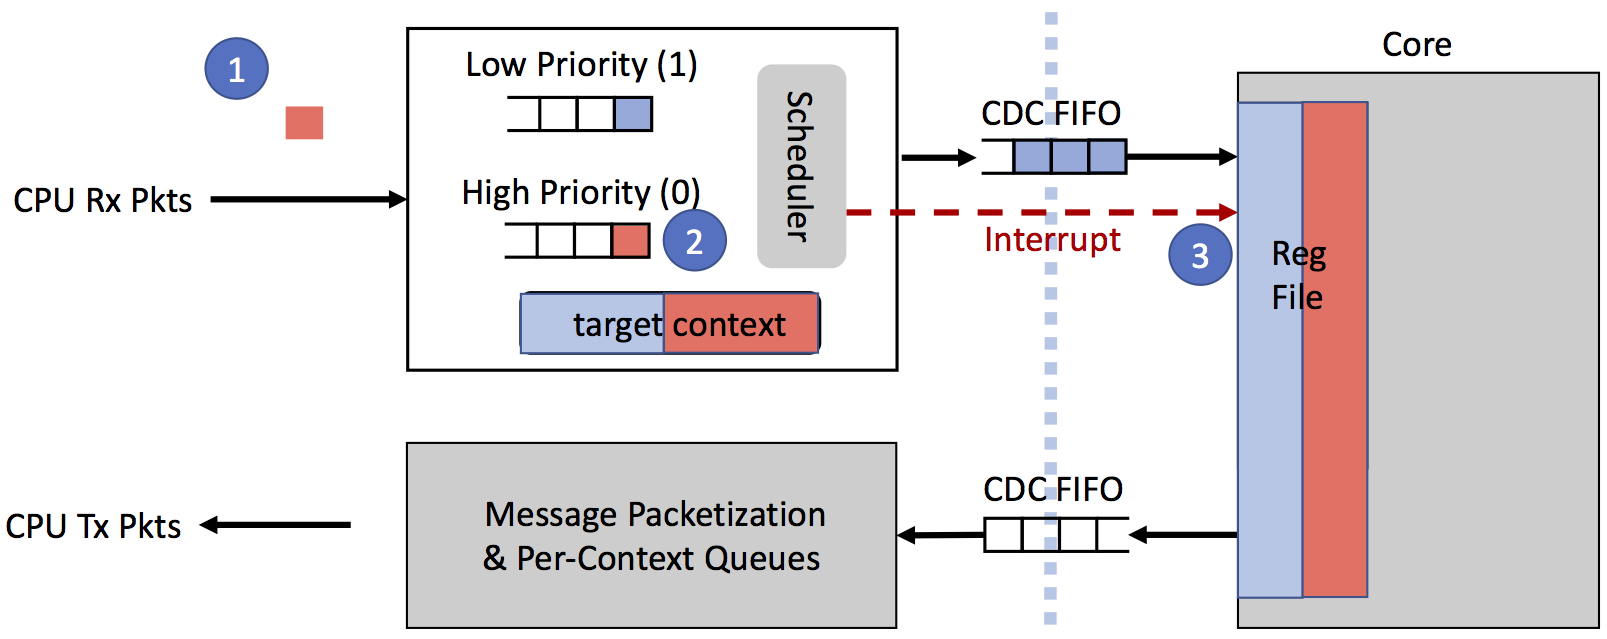
\includegraphics[width=\linewidth]{./figures/nic-scheduler}
  \caption{The steps that occur when a low priority thread is running on the core and then a message arrives for a higher priority context.}
  \label{fig:nic-scheduler}
\end{figure}